\setchapterpreamble[u]{\margintoc}
\chapter{Generation of infrared point clouds}
\labch{thermal_pc}
\label{sec:thermal_pc}

\section*{About this chapter}

This chapter describes the generation of dense thermographic point clouds by mapping image datasets into large RGB point clouds. The GPU hardware is used to accomplish these time-consuming tasks with low response time, outperforming currently available approaches for generating thermal point clouds. Occlusion and visibility tests are addressed for projecting accurate thermal data, together with the use of penalty and aggregation functions. Finally, the generated point cloud is applied to the thermal characterization of vegetation. The complete workflow of this methodology is shown in Figure \ref{fig:thermal_projection_overview}.

The proposed methodology overcomes the current state-of-the-art drawbacks on the reconstruction of thermal point clouds. The solution is implemented from scratch, thus enabling low-level optimizations and taking advantage of GPU capabilities. Firstly, a baseline point cloud is reconstructed through SfM-MVS and high-resolution RGB imagery. Consequently, large and dense point clouds are the input of the approach that is later explained. Then, co-acquired RGB and thermal image datasets are registered, and the subsequent projection of a 3D point cloud into the RGB-thermal image space is performed by addressing the geometric properties of the scene. a viable geometrical description of the scene. Furthermore, the use of several aggregation functions that minimize the distance from aggregated values (3D point cloud) to image samples is evaluated. The outcome is a dense thermal point cloud that preserves image details.

The full source code is available at\newline \url{https://github.com/AlfonsoLRz/RGBThermalFusion}.

\section{On the generation of thermal point clouds}

Infrared radiation provides valuable data that enable detecting and describing the scene surfaces. It comprises a wide range of applications, from quality control and monitoring in industrial environments \cite{alfredo_osornio-rios_recent_2019}, to building inspection \cite{jarzabek-rychard_supervised_2020} as well as agriculture and animal applications \cite{tsouros_review_2019}. The acquisition of high-resolution UAV-based imagery provides an opportunity to estimate three-dimensional models from a scene, such as point clouds or digital surface models (DSM). 3D models in \gls{Remote sensing} are mainly achieved by using laser sensors, e.g., LiDAR \cite{yandun_narvaez_survey_2017}, and photogrammetry. 

Furthermore, 3D representations of surveyed environments have been gaining interest \cite{jurado_remote_2022}. Firstly, interaction with 3D environments speeds up the tasks of human operators such as detecting building failures \cite{lin_fusion_2019}. Also, the results of 3D reconstructions are much more valuable and informative for the client counterpart. Finally, it reduces the analysis of multiple datasets into a single one where comparisons are effectively performed. Among 3D representations, point clouds have been significantly preferred over mesh models as they do not involve the reconstruction of surveyed surfaces \cite{park_comparison_2019} into polygons. Instead, a discretized version is provided, though its rendering has been proved to achieve nearly mesh-like results with modern hardware and large point clouds \cite{schutz_rendering_2021}.   

As previously stated in Section \nameref{sec:fundamentals_rs}, SfM relies on pixel data for finding key points that can be detected in several images. Therefore, estimating 3D point clouds from low-resolution thermal imagery is challenging. First, these present more substantial noise in comparison with RGB images \cite{sledz_thermal_2018} as well as aberration-induced blurring which causes the spreading of the object radiance. Consequently, the number of extracted tie points in thermography images is smaller, and the resulting 3D point clouds are much sparser and less accurate \cite{jarzabek-rychard_supervised_2020}. The outcome is proven to improve if further calibration is considered \cite{ribeiro-gomes_uncooled_2017}; however, identifying GCPs in thermography may be challenging because of the material appearance and radiance spreading \cite{javadnejad_photogrammetric_2020}. All these shortcomings also worsen the performance of naive fusion approaches, such as the alignment of RGB and thermographic point clouds with methods such as ICP. 

Table \ref{table:thermal_pc_attributes} shows the nomenclature of the parameters used in this work. Some of them are calculated by the SfM-MVS algorithm, whereas others are extracted from the device specifications.

\begin{figure*}
    \centering
    \caption{Summary of the procedure of this work. SfM-MVS and image registration stages build isolated results and thus can be performed in parallel. Thermal information is assigned to 3D points by considering the point cloud occlusion and selecting an appropriate aggregation operator that reduces the error from image samples to the outcome. The visualization of the resulting point cloud is improved by highlighting outlier values. Finally, the vegetation is identified and characterized through its temperature. }
    \label{fig:thermal_projection_overview}
    \includegraphics[width=\linewidth]{figs/thermal_projection/thermal_projection.png}
\end{figure*}

\section{Estimation of RGB point clouds}

RGB point clouds were estimated with SfM-MVS using high-resolution RGB images through methods. Several open-source and commercial software integrate this algorithm and therefore it is trivial to obtain, regardless of the achieved precision. In this work, Pix4Dmapper was used, and the estimation algorithm was further optimized through the marking of GCPs. The density and storage size of the result depends on the image resolution. Therefore, this parameter can be adjusted while dealing with occlusion problems in the point cloud.

\renewcommand{\arraystretch}{1.15}
\begin{table*}
    \caption{Parameters obtained both from RGB and thermal camera calibration and image metadata.}
    \label{table:thermal_pc_attributes}
    \begin{tabular}{@{}ll@{}}
    \toprule
    Parameter & Definition\\
    \midrule
    Image size ($w_{\textit{image}}, h_{\textit{image}}$) & Original image size.\\
    Principal point ($c_x$, $c_y$) & Intersection of the principal axis and the image plane. \\
    Focal length ($f_x$, $f_y$) & Distance in pixels from the centre of projection and the image plane. \\
    Sensor width and height ($w_{\textit{sensor}}, h_{\textit{sensor}}$) & Size in millimeters (\si{\milli\meter}). \\
    Omega, Phi, Kappa ($\omega, \phi, \kappa$) & Rotation between the image coordinate system and the world system. \\
    Camera position ($t_{\textit{local}}$) & Camera position in the point cloud system.\\
    World offset ($t_{\textit{world}}$) & Offset between the local coordinate system and the UTM system.\\
    Camera matrix ($K$) & Calculated from previous parameters as $\begin{pmatrix} f_x & 0 & c_x\\ 0 & f_y & c_y\\ 0 & 0 & 1\\ \end{pmatrix}$ \\
    Rotation matrix ($R$) & Composition of $R(\omega)R(\phi)R(\kappa)$. \\
    Projection matrix ($P$) & Distortion-free projection in a pinhole model: $K \cdot \begin{bmatrix} R|-Rt_{\textit{local}} \end{bmatrix}$. \\
    Radial distortion coefficients ($k_1, k_2, k_3$) & Distortion coefficients, mostly visible on straight lines.\\
    Tangential distortion coefficients ($p_1, p_2$) & Misalignment of device lens with respect to the image plane. \\
    \bottomrule
    \end{tabular}
\end{table*}
\renewcommand{\arraystretch}{1}    

\section{Image matching}

The fusion of RGB point clouds with thermal data can be performed through a first step based on image registration. This approach tackles those challenges derived from estimating thermal point clouds directly. Hence, the processing tasks are carried out on a single 3D point cloud, e.g., marking GCPs. To this end, 3D RGB points are projected into the RGB image plane as shown in Equation \ref{eq:thermal_projection}:
\begin{gather}
    \label{eq:thermal_projection}
    \begin{aligned}
        \begin{bmatrix} x^\prime, y^\prime, z^\prime \end{bmatrix}^\intercal = P \begin{bmatrix} x, y, z\end{bmatrix}^\intercal
        \begin{bmatrix} x'', y'' \end{bmatrix}^\intercal = \frac{1}{z^\prime} \begin{bmatrix} x^\prime, y^\prime \end{bmatrix}^\intercal
    \end{aligned}
\end{gather}
provided that $\begin{bmatrix} x, y, z\end{bmatrix}$ is expressed in the local coordinate system where both the point cloud and the cameras are defined. Otherwise, if defined in a global coordinate system such as UTM:
\begin{gather}
    \label{eq:thermal_projection_2}
    \begin{bmatrix} x, y, z \end{bmatrix}^\intercal = \begin{bmatrix} x_{\textit{global}}, y_{\textit{global}}, z_{\textit{global}} \end{bmatrix}^\intercal - t_{\textit{world}}
\end{gather}

Consequently, each 3D point is linked to two values, $x'', y'' \in \mathbb{R}$, for each image. Note that $t_{\textit{world}}$ is defined as an arbitrary shift of real-world points to avoid working with large values. The same reasoning applies to the local positions of cameras, $t_{\textit{local}}$. The matching of RGB and thermal datasets were achieved using ECC, thus expressing the misalignment of two images with a homography matrix, $H_i$, of size $3\times3$.

The procedure for applying ECC to RGB and TIR images starts by cropping each RGB image. However, the homography matrix $H_i$ also involves rotations and thus the area to be cropped must be expressed using a rectangle centred at $(\frac{w_{\textit{image}}}{2}, \frac{h_{\textit{image}}}{2})$. It ensures covering thermal images in every possible configuration. With this approach, RGB images are defined as source images, while thermographic images are transformed to align both of them. The computed homography matrix projects thermal images into cropped RGB images as shown in Equations \ref{eq:thermal_projection} and \ref{eq:thermal_projection_2}, whereas the inverse matrix performs the backward projection. 

\begin{marginfigure}[.1cm]
	\includegraphics{figs/thermal_projection/thermal_ecc_registration.png}
	\caption{A sample of matching RGB and thermal images. The latter is overlapped within the RGB image and depicted with transparency ($\alpha = 0.7$). The bottom image presents the final quadrilateral shape. }
	\label{fig:thermal_ecc_registration}
\end{marginfigure}
In summary, $C_{i} \cdot \inv{H_i}$ projects 2D RGB points into a thermal image, provided that $C_{i}$ is a composite matrix (Equation \ref{eq:cropping_composite_matrix}) that defines the inverse cropping transformation. Note that projected points may fall out of the thermal image boundaries and a point in polygon test must be carried out. It is very simple to perform in this work since the inverse homography matrix $\inv{H_i}$ leads to an ideal rectangle, and thus only four Boolean operations are required.  
\begin{gather}
    \label{eq:cropping_composite_matrix}
    \begin{aligned}
        C_{i} = & \hspace{1mm} T_{\textit{crop}} * S_{\textit{ratio}} * T_{-\textit{center}_{\textit{RGB}}} =\\
           = &\begin{bmatrix}
                        1 & 0 & \frac{w_{\textit{thermal}_u}}{2}\\
                        0 & 1 & \frac{h_{\textit{thermal}_u}}{2}\\
                        0 & 0 & 1
                    \end{bmatrix} \cdot 
                    \begin{bmatrix}
                        r_x & 0 & 0\\
                        0 & r_y & 0\\
                        0 & 0 & 1
                    \end{bmatrix} \cdot
                    \begin{bmatrix}
                        1 & 0 & -\frac{w_{\textit{RGB}_u}}{2}\\
                        0 & 1 & -\frac{h_{\textit{RGB}_u}}{2}\\
                        0 & 0 & 1
                    \end{bmatrix} =\\
                    = &\begin{bmatrix}
                        r_x & 0 & \frac{1}{2}(-r_{x} w_{\textit{RGB}_u} + w_{\textit{thermal}_u})\\
                        0 & r_y & \frac{1}{2}(-r_{y} h_{\textit{RGB}_u} + h_{\textit{thermal}_u})\\
                        0 & 0 & 1
                    \end{bmatrix}\\
        (r_x, r_y) = & \hspace{1mm} \left(\frac{\textit{crop}_x}{w_{\textit{thermal}_u}}, \frac{\textit{crop}_y}{h_{\textit{thermal}_u}}\right)
    \end{aligned}
\end{gather}
where ($\textit{crop}_x$, $\textit{crop}_y$) are the dimensions of the cropped area, ($w_{\textit{thermal}}, h_{\textit{thermal}}$) are the dimensions of undistorted thermal images and \textit{u} subscript refers to the indices of undistorted images. Figure \ref{fig:thermal_ecc_registration} shows the result of the registration methodology as well as the warped quadrilateral shape.

Composite matrices $C_i$ were calculated once and stored in binary files to avoid repeating this time-consuming for every application launch. Some pairs of images may not be matched, and in those cases, the ECC algorithm either fails to converge or the resulting quadrilateral shape is very distorted. Detecting the second undesired scenario required defining a strict threshold based on the degrees of the minimum/maximum angles after transforming a rectangle shape. Still, 3D points were more likely to be visible in multiple images as the drone flight mission was planned with a high overlapping factor. Table \ref{table:image_registration_statistics} shows the percentage of thermal images which could be matched to RGB images as well as the number of 3D points that were not visible from any registered thermal image. Remark that the FOV is wider for the RGB device and thus edge points refer to points that were not visible in any thermal images, regardless of the matching results. Hence, it was observed that every unregistered point was not visible from any viewpoint and all of them were located on the edges. For larger point clouds, the number of edge points grows unevenly with respect to the rest of the scenario, thus decreasing the percentage of unregistered and edge points.

\begin{table}
    \caption{a) Percentage of pairs of RGB-thermal images that were successfully matched, and b), percentage of points which were not visible from any thermal image for two different point clouds. Edge points refer to points that were not visible even if the complete image dataset was successfully registered. A large radius ($r \gets 80$\si{\meter}) was utilized during the search of candidate points to avoid omitting visible values.}
    \label{table:image_registration_statistics}
    \begin{tabular}{l@{\hskip 0.5in}l@{}}
        \multicolumn{2}{c}{a) 2D}\\
        \midrule
        \textbf{\#Images} & \textbf{Registered}\\
        \midrule
        410 & 89,7561\% \\
        \bottomrule
    \end{tabular}\\[2mm]
    \begin{tabular}{l@{\hskip 0.5in}l@{\hskip 0.5in}l@{}}
        \multicolumn{3}{c}{b) 3D}\\
        \midrule
        \textbf{\#Points} & \textbf{\#Non-registered} & \textbf{\#Edge points}\\
        \midrule
        19.161.076 & 18,8952\% & 100\% of 18,8952\%\\
        98.016.324 & 15,5823\% & 100\% of 15,5823\%\\
        \bottomrule
    \end{tabular}
\end{table}

\section{Thermal image mapping}

Merging RGB and thermography data was performed with the previously cited projection. First, a naive approach that neither considered occlusion nor visibility was implemented. As a result, thermal data were mapped to 3D points as long as they were visible from any thermal viewpoint. Equation \ref{eq:thermal_projection} enables projecting each 3D point into the RGB image plane. Points were considered not visible from a viewpoint and thus discarded if their projected coordinates had values smaller than zero or larger than the dimensionality of RGB images. In addition, the image matching imposes another rejection condition due to the smaller thermal FOV. 2D coordinates within thermal images ($x_{\textit{thermal}}, y_{\textit{thermal}} \in \R$) were sampled using a bilinear interpolation in which surrounding pixels also affect the outcome. The weight factors were given by their distance to ($x_{\textit{thermal}}, y_{\textit{thermal}}$). The projected values were aggregated using the arithmetic mean as the default approach.

\begin{marginfigure}[.0cm]
	\caption{Rendering of a) an octree whose nodes are spheres, optimized for searches within a radius, and b) a traditional octree whose nodes are boxes. }
	\label{fig:point_cloud_octrees}
	\includegraphics{figs/thermal_projection/octrees.png}
\end{marginfigure}
The main challenge of this step is to search for candidate points for every image. Points are not assumed to be uniformly sparsed and thus using regular grids was discarded. Instead, the point cloud was managed with an octree optimized for searching neighbours within a radius \cite{behley_efficient_2015}. A radius search is preferred over a box search since previous corrections involve interpolations that leave more imprecise values at the boundaries. This data structure organizes the 3D RGB points instead of the array of image viewpoints; otherwise, an efficient search would not be needed due to the relatively low number of images. The search radius is significantly easier to define whether it is expressed at ground level as $(x, aabb_{\textit{center}_{y}}, z)$, given that $x$ and $z$ depend on the local position of the image viewpoint and $aabb_{\textit{center}_{y}}$ is the $y$-axis coordinate for the center of the axis-aligned bounding box (AABB) of the environment. Figure \ref{fig:point_cloud_octrees} renders the described data structure and a conventional octree. Finally, Figure \ref{fig:thermal_point_cloud_top_view} shows a top view of the reconstructed thermal point cloud.

\begin{figure}[ht]
	\centering
	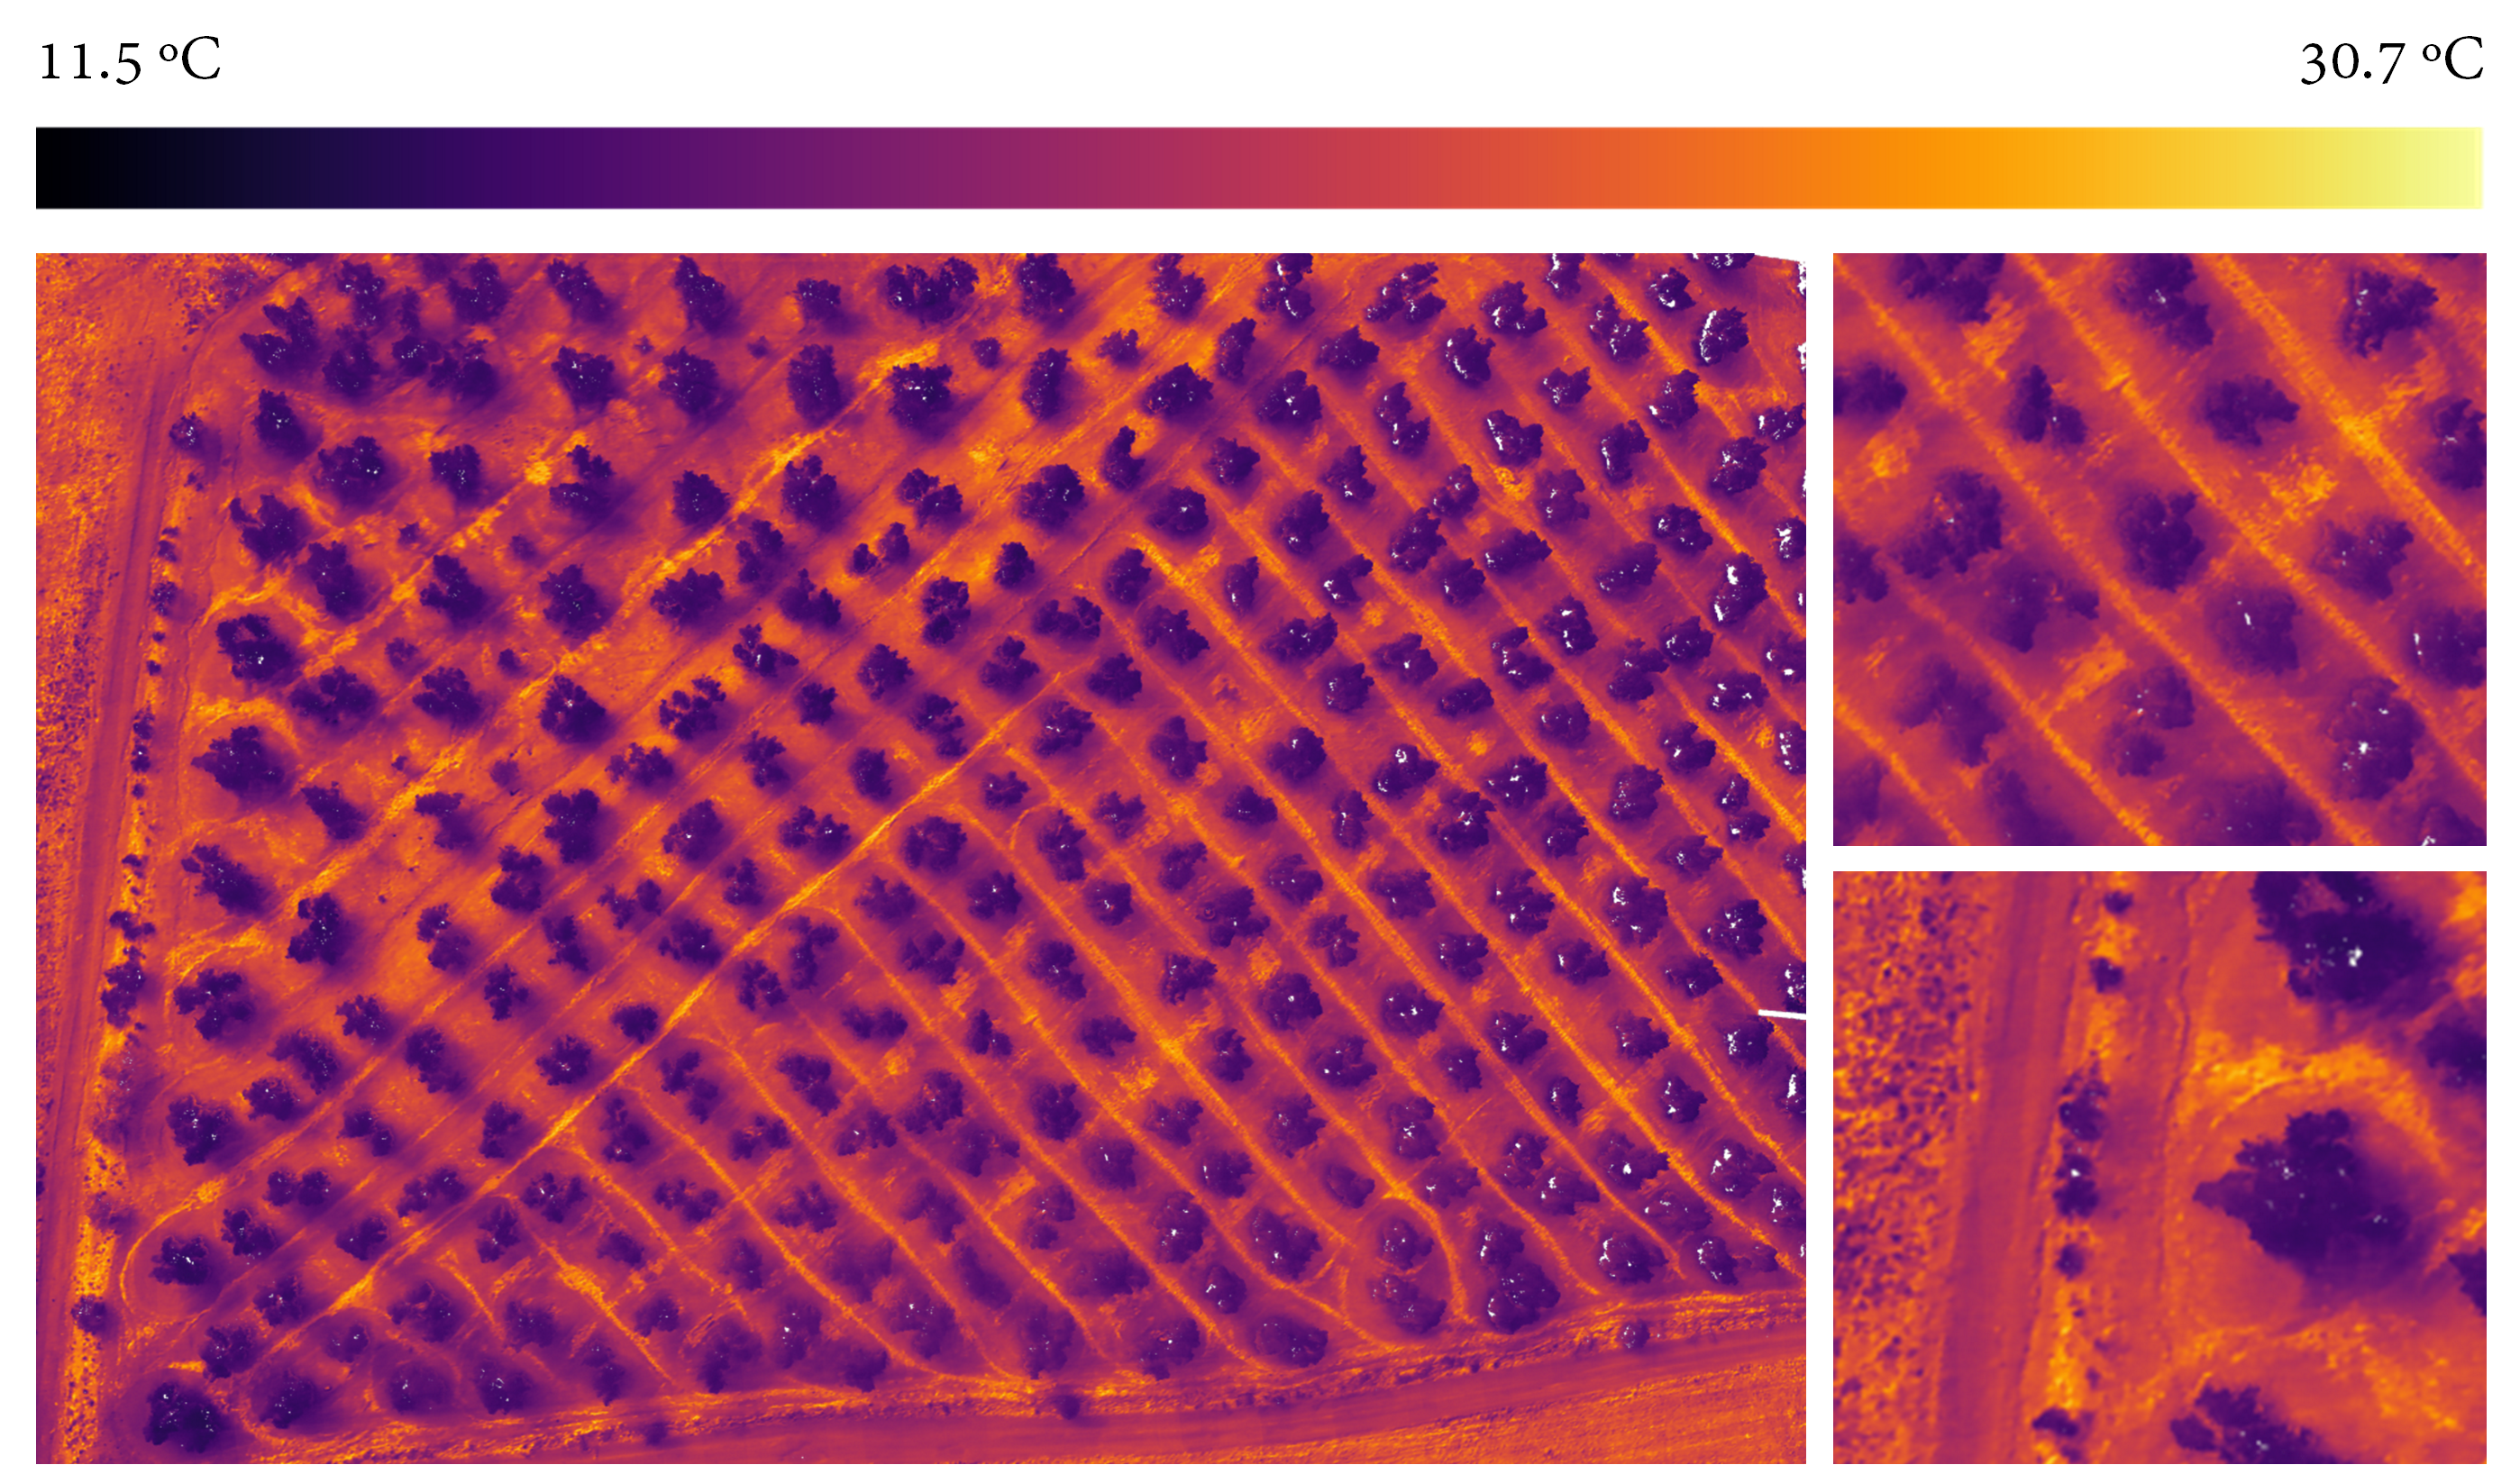
\includegraphics{figs/thermal_projection/thermal_inferno_temperature.png}
	\caption{Top view of a thermal point cloud captured by a nadir camera. Absolute temperature values are normalized and mapped to the upper texture. The search radius was fixed to 30 \si{\meter}.}
	\label{fig:thermal_point_cloud_top_view}
\end{figure}

\section{Occlusion}

Although the previous methodology presents a valid and comprehensible approach for reconstructing thermal point clouds, it can be called an imprecise intensity projection. Occluded points ought not to obtain data from foreground objects, and this has been previously solved by ray-casting voxelized environments \cite{vidas_real-time_2015}. However, this solution lacks accuracy and flexibility since octrees are mainly constructed with top-down methodologies. Therefore, the size of a voxel depends on the subdivision of the point cloud bounding box, either using a maximum depth or a maximum number of primitives in a single node. At least two approaches are following proposed to solve this challenge. Both lead to point clouds where the number of thermal values to be aggregated over each 3D point is lower, although these are ensured to be more valuable and precise.

\subsection{Visibility test}

\begin{marginfigure}[.0cm]
	\includegraphics{figs/thermal_projection/depth_buffer.png}
	\caption{Depth buffer of a camera during a visibility test carried out with a radius of size a) 20\si{\meter} and b) 30\si{\meter}.}
	\label{fig:depth_buffer}
\end{marginfigure}
Images are discrete representations from where the SfM-MVS algorithm can estimate at least one 3D point from every RGB pixel. A depth buffer (or \textit{z}-buffer) of the same size as the resolution used during the point cloud estimation can be constructed for each image. Still, this size can be increased to build a sub-pixel level method. In this approach, the index of the closest 3D point is stored for every viewpoint and pixel within it along with the minimum depth ($\textit{z}$). The latter determines if a point could be visible. Depth buffers were represented as sparse matrices to reduce the memory footprint and implemented as a hash map that stores pairs of values. Keys were the access index of a 2D point and values represented the nearest point for such a position. A depth buffer is depicted in Figure \ref{fig:depth_buffer}, showing a circular pattern as a result of the search algorithm. The workflow for determining which points are visible is presented in Algorithm \ref{alg:depth_buffer_test}.  

\begin{algorithm}
	\caption{Visibility test to accurately map thermal images into an RGB point cloud. }
	\label{alg:depth_buffer_test}
    \begin{algorithmic}[1]
        \State \textbf{Input} RGB point cloud: $P$
    	\State \textbf{Input} RGB images: $c$
    	\State \textbf{Input} RGB resolution during SfM-MVS procedure: ($w_{\textit{SfM}}, h_{\textit{SfM}}$)
    	\State \textbf{Input} Search radius: $R$
        \State \textbf{Output} Array of normalized and absolute thermal values.
		\For {Every image $c_i$ captured from the position $p_{c_{i}}$}
		    \State Create a new buffer of size ($w_{\textit{SfM}}, h_{\textit{SfM}}$) with $d_{x,y} = \infty$ provided that $0 \leq x < w_{\textit{SfM}}$ and $0 \leq y < h_{\textit{SfM}}$.
		    \State Retrieve candidate points within the radius \textit{R} through the point cloud octree
		    \For {Every three-dimensional candidate point $p_j$}
		        \State Calculate 2D TIR point $(x, y)$ (Eq.: \ref{eq:thermal_projection})
		        \If {$(x, y)$ in TIR polygon}
		            \If {$\textit{distance}(p_{c_{i}}, p_j) < d_{x, y}$}
		                \State Add point to depth buffer and update the minimum distance found at $d_{x, y}$
	    	        \EndIf
	    	    \EndIf
		    \EndFor
		    \For {Every point $p_j$ stored in depth buffer}
		        \State Retrieve and accumulate the normalized and absolute thermal values from $c_i$ for $p_j$
		    \EndFor
		\EndFor
		\State Compute final values for each point of $P$ as an arithmetic mean
	\end{algorithmic} 
\end{algorithm}

\newpage
\subsection{Occlusion test}

\begin{marginfigure}[.0cm]
	\centering
	\includegraphics{figs/thermal_projection/triangle_mesh_reconstruction_zoom.png}
	\caption{Triangle mesh estimated for a point cloud subset through Advancing Front algorithm. Reconstruction of vegetation is clearly erroneous in comparison with the ground.}
	\label{fig:advancing_front_mesh}
\end{marginfigure}
Occlusion tests can be performed with ray-casting as long as the target scenario is represented as a triangle mesh. However, estimating the mesh from a point cloud is challenging. Multiple algorithms are found in the bibliography; some require the normal vector, while others are robust enough to work without surface orientation, e.g., Advancing Front reconstruction \cite{cohen-steiner_greedy_2004}. However, surface reconstructions are time-consuming algorithms that rely on multiple parameters whose values are not trivial to define. Additionally, reconstructing vegetation is more likely to fail since leave modelling is very intricate. Figure \ref{fig:advancing_front_mesh} shows the result of Advancing Front surface reconstruction for a subset of RGB points. Faces were oriented considering that the viewpoint is above the scene. Hence, faces were flipped if $\hat{n} \cdot \widehat{(v - p)} > \frac{\pi}{2}$, provided that $\hat{n}$ is the surface normal, $v$ is an image viewpoint and $p$ is a 3D point over the triangle mesh surface. A schematic representation of the occlusion methodology is depicted in Figure \ref{fig:occlusion_overview}.

On the other hand, points could be determined as occluded or not if they had a volume. This assumption enables solving this task with ray-casting, and despite it being time-consuming, there are data structures optimized for rapidly discarding large parts of the scene. For instance, a Bounding Volume Hierarchy (BVH) is a tree structure where each primitive of the scene is bounded by an AABB, whereas surrounding AABBs are merged up to the tree root. Better cluster separations lower the trace time as they reduce the number of steps until reaching the target leaf node. In this work, point volumes were modelled as spheres that provided an efficient alternative to viewpoint-oriented boxes. Their radius was calculated relative to the viewpoint altitude (Figure \ref{fig:occlusion_overview}), as shown in Equation \ref{eq:gsd_radius_equation}. It represents an efficient and flexible approach, while the intersection test of a ray with an oriented bounding box (OBB) is slightly more complex.
\begin{equation}
    \label{eq:gsd_radius_equation}
    R = \frac{\frac{w_{sensor} \cdot height}{f_x \cdot w_{image}}}{2} = \frac{\frac{h_{sensor} \cdot height}{f_y \cdot h_{image}}}{2} = \frac{\textit{GSD}}{2}
\end{equation}
with \textit{GSD} being the Ground Sample Distance, i.e, the size of a pixel if the camera is at an altitude of \textit{height}. \textit{R} is defined in \si{\meter}/pixel, despite $w_{sensor}$ and $f_x$ being defined in \si{\milli\meter}.

\begin{marginfigure}[.0cm]
	\centering
	\includegraphics{figs/thermal_projection/occlusion_spheres.png}
	\caption{Occlusion test with two points represented as spherical volumes. a) Point where the ray impacts first ($p_1$), occluding b) the point $p_2$.}
	\label{fig:occlusion_overview}
\end{marginfigure}
Spherical volumes may vary for each 3D point and image viewpoint, thus requiring building a BVH for every viewpoint and  subset of candidate points. However, they were constructed using the GPU hardware to speed up this task as proposed by Meister and Bittner \cite{meister_parallel_2018}. Primitives were ordered using their Morton codes (30 bits representing \textit{xyz} coordinates) and subsequently merged by efficiently searching the nearest neighbour, which also happens to be in a close index of the sorted buffer. On the other hand, the ray-casting was also solved on GPU by generating a ray for each 3D point; rays from occluded points collided with a closer volume, and those belonging to visible points did not find any closer volume (Figure \ref{fig:occlusion_overview}). The pseudocode of this methodology is illustrated in Algorithm \ref{alg:occlusion_test}.

\begin{algorithm}[hbt]
	\caption{Occlusion test to determine temperature values of sphere-shaped RGB points with adaptive radius.}
	\label{alg:occlusion_test}
	\begin{algorithmic}[1]
    	\State \textbf{Input} RGB point cloud: $P$ %\;
    	\State \textbf{Input} RGB images: $c$ %\;
    	\State \textbf{Input} Search radius: $R$ %\;
        \State \textbf{Output} Array of normalized and absolute thermal values. %\;
		\For {Every image $c_i$ captured from the position $p_{c_{i}}$}
		    \State Retrieve candidate points within the radius \textit{R} through the point cloud octree %\;
		    \State Build a new BVH with the array of candidate points %\;
		    \Procedure{Sort points}{}
		        \State Sort candidate points expressed as Morton codes and build BVH leaves %\;
		        \State Join leaf and intermediate nodes while root is not reached %\;
		    \EndProcedure
		    \For {Every three-dimensional candidate point $p_j$}
		        \State Throw rays from every point and find the first intersected volume %\;
		        \If {Intersected volume = $volume_{p_j}$}
		            \State Calculate 2D TIR point $(x, y)$ (Eq.: \ref{eq:thermal_projection}) %\;
		            \If {$(x, y)$ in TIR polygon}
		                \State Retrieve and accumulate the normalized and absolute thermal values from $c_i$ for $p_j$ %\;
	    	        \EndIf
	    	    \EndIf
		    \EndFor
		\EndFor
		\State Compute final values for each point of $P$ as an arithmetic mean %\;
	\end{algorithmic} 
\end{algorithm} 

\section{Visualization}

Javadnejad et al. \cite{javadnejad_photogrammetric_2020} proposed to visualize thermal data by linearly interpolating RGB and thermographic data. RGB colours were converted to grayscale and temperature values were mapped to an RGB value through a colour-ramp function. The weight, $w(t)$, was computed as the distance of each temperature sample, $t$, to the mean, $t_{mean}$, so that $w(t) = 1$ omits RGB colours. Although it accentuates cold and hot regions ($w(t) \gets 1$), intermediate values were also merged with grayscale colours. Therefore, the representation of non-anomalous temperature values distorted the colour distribution of the RGB point cloud and did not help with anomaly identification.

Instead, outlier values can be identified using a conventional numeric outlier method. To this end, thermal values were sorted in GPU to retrieve first and third quartiles, $Q_1$ and $Q3$, as well as the interquartile range (\textit{IQR} $\gets Q3 - Q1$). Values under $Q_1 - k$(\textit{IQR}) and above $Q3 + k$(\textit{IQR}), where $k \geq 0$, were considered to be anomalous values and thus $w(t)$ was assigned to $1$. The visualization of intermediate values was computed as proposed by Javadnejad et al. \cite{javadnejad_photogrammetric_2020}. However, RGB colours were not converted to grayscale nor we utilized a linear interpolation. Instead, a Hermite interpolation was used to emphasize values of $t$ close to $t_{\textit{min}}$ and $t_{\textit{max}}$. 

\begin{figure}[ht]
	\centering
	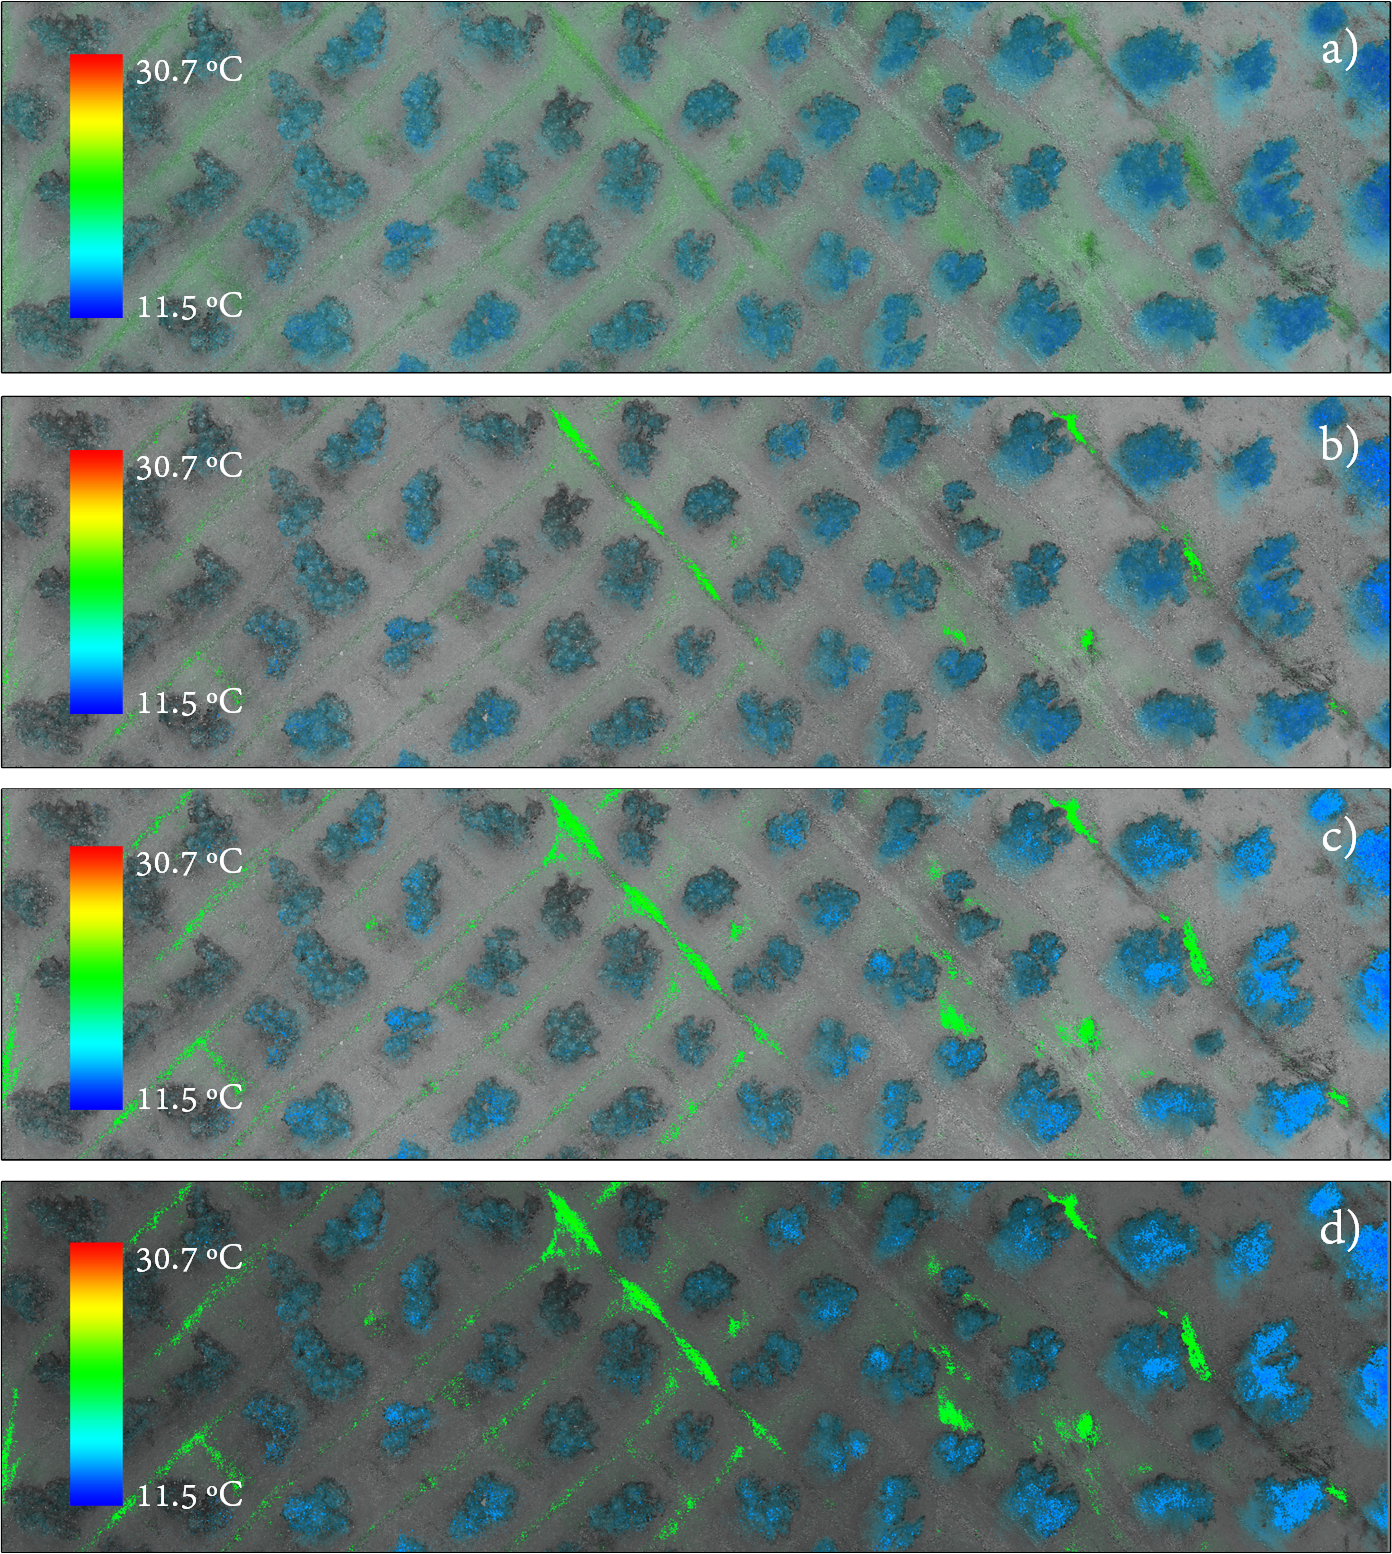
\includegraphics{figs/thermal_projection/visualization_thermal_anomalies.png}
	\caption{Visualization of the study area using multiple configurations. a) Visualization proposed by Javadnejad et al. \cite{javadnejad_photogrammetric_2020}, while b), c) and d) show our modified procedure. b) $\gamma = 0.8, k = 0.8$, c) $\gamma = 0.8, k = 0.5$, d) $\gamma = 0.5, k = 0.5$.}
	\label{fig:visualization_thermal_anomalies}
\end{figure}

Equation \ref{eq:blending_function} shows the procedure for computing the proposed enhanced visualization. Note that $\gamma$ enables modifying the brightness of RGB colours, where $0 \leq \gamma \leq 1$. Figure \ref{fig:visualization_thermal_anomalies} depicts the use of $\gamma$ to darken irrelevant regions. On the other hand, $\zeta(t)$ represents a colour mapping function that is also parameterized by the temperature. In this work, $\zeta(t)$ is given by the texture depicted at the left side of Figure \ref{fig:visualization_thermal_anomalies}.
\begin{gather}
    \label{eq:blending_function}
    \begin{aligned}
        \begin{bmatrix}
            r'\\g'\\b'
        \end{bmatrix} &=
        H(w(t))\zeta(t) + \gamma(1 - H(w(t)))\begin{bmatrix}
            r\\g\\b
        \end{bmatrix}\\
        w(t) &=
        \begin{cases}
            1 &t_{min} \leq t < Q_1 - k(\textit{IQR})\\
            \frac{t_{mean} - t}{t_{mean} - t_{min}} &Q_1 - k(\textit{IQR}) \leq t \leq t_{mean}\\
            \frac{t - t_{mean}}{t_{max} - t_{mean}} &t_{mean} < t \leq Q_3 + k(\textit{IQR})\\
            1 &Q_3 + k(\textit{IQR}) < t < t_{max}
        \end{cases}\\
        H(w(t)) &=
        \begin{cases}
            w(t) &w(t) = 1\\
            w(t)^2(3 - 2w(t)) &\text{otherwise}
        \end{cases}
    \end{aligned}
\end{gather}

\section{Aggregation of image samples}

\begin{marginfigure}[.0cm]
	\includegraphics{figs/thermal_projection/brdf_thermal.png}
	\caption{Representation of a point cloud with 19 TIR radiation samples observed from different viewpoints for the same surface point. Sampled emission values are compared to a Lambertian radiator (semisphere). }
	\label{fig:brdf_thermal_samples}
\end{marginfigure}
3D points are mapped to several images and therefore, these may receive many thermal measurements, with all of them being valid regardless of being different. The frequent approach is to average them with the arithmetic mean \cite{javadnejad_photogrammetric_2020}, although it could be especially sensitive to extreme values. Figure \ref{fig:brdf_thermal_samples} depicts 19 thermal samples that were aggregated in a single 3D point. A different approach is to consider multiple aggregation functions that can be either used separately or combined. When combined, their outputs are compared to a set of inputs that help in selecting the aggregation that minimizes the outcome of a penalty function. Consequently, the penalty function determines the similarity of each aggregation output to a set of thermal samples.

Previously stated aggregation definitions are considerably simplified in this work since data is 1D ($n = 1$). Therefore, we simply needed to define a collection of aggregation and penalty functions, such as the following.
\begin{itemize}
    \item Minimum: $f(x) = \underset{i}{\argmin}\, x_i$
    \item Maximum: $f(x) = \underset{i}{\argmax}\, x_i$
    \item Arithmetic mean: $f(x) = \frac{\sum_{i=1}^{n} x_i}{n}$
    \item Geometric mean: $f(x) = \sqrt[n]{\prod_{i=1}^{n} x_i}$
    \item Harmonic mean: $f(x) = n\left( \sum_{i=1}^{n} \frac{1}{x_i} \right)^{-1}$
\end{itemize}
whereas penalty functions are less intricate as their objective is to measure the error between the inputs and the aggregated value, $y$. On the other hand, three penalty functions \cite{paternain_color_2012} were considered for minimizing the dissimilarity of new results and input samples. 
\begin{itemize}
    \item $P_1(x_i, y) = \abs{x_i - y}$
    \item $P_2(x_i, y) = (x_i - y)^2$
    \item $P_3(x_i, y) = \abs{x_i - y}^3$
\end{itemize}

The frequency on which every aggregation function was selected was measured for three different penalty functions, $P(x_i, y)$. Table \ref{table:thermal_aggregation_frequency} shows the preference ratio of three local penalty functions against five aggregation operators. The arithmetic mean is the preferred aggregation, despite geometric and harmonic means being also widely used. Maximum and minimum operators were barely utilized, and their highest frequency was observed for occlusion-based approaches that handle a lower number of samples. Consequently, the number of operators could be reduced by discarding seldom aggregations, thus enabling a faster selection.

\renewcommand{\arraystretch}{1.2}
\begin{table*}
    \centering
    \caption{Preference ratio of each aggregation operator over three different penalty functions. Frequency is normalized in $[0, 1]$, and therefore the sum of each row is one. The first and second preferred choices for each configuration are highlighted in bold. }
    \label{table:thermal_aggregation_frequency}
    \begin{tabular}{@{}llccccc@{} }
    \toprule
    & & \multicolumn{5}{c}{\textbf{Aggregation functions}} \\
    \cmidrule{3-7}
    Penalty function & Approach & Arithmetic $\mu$ & Geometric $\mu$ & Harmonic $\mu$ & Max & Min\\
    \midrule
    \multirow{2}{*}{$g_1 : \underset{y}{\mathrm{argmin}}\, \sum_{i=1}^{n} \abs{x_i - y}$} & Naive & \textbf{0.64699} & 0.07563 & \textbf{0.23348} & 0.02530 & 0.01858 \\
    & Depth buffer & \textbf{0.65672} & 0.06017 & \textbf{0.21589} & 0.03815 & 0.02905 \\
    & Occlusion & \textbf{0.67193} & 0.03362 & \textbf{0.17048} & 0.07004 & 0.05392 \\
    \multirow{2}{*}{$g_2 : \underset{y}{\mathrm{argmin}}\, \sum_{i=1}^{n} (x_i - y)^2$} & Naive & \textbf{0.67787} & \textbf{0.15036} & 0.14783 & 0.01312 & 0.01080 \\
    & Depth buffer & \textbf{0.66193} & 0.13732 & \textbf{0.16330} & 0.02067 & 0.01676 \\
    & Occlusion & \textbf{0.63223} & 0.10407 & \textbf{0.19052} & 0.03972 & 0.03344 \\
    \multirow{2}{*}{$g_3 : \underset{y}{\mathrm{argmin}}\, \sum_{i=1}^{n} \abs{x_i - y}^3$} & Naive & \textbf{0.57092} & 0.14996 & \textbf{0.25392} & 0.01412 & 0.01106 \\
    & Depth buffer & \textbf{0.56471} & 0.13513 & \textbf{0.26142} & 0.02171 & 0.01701 \\
    & Occlusion & \textbf{0.57647} & 0.09821 & \textbf{0.25101} & 0.04057 & 0.03371 \\
    \bottomrule
    \end{tabular}
\end{table*}
\renewcommand{\arraystretch}{1}

\section{Thermal characterization of vegetation}

Analyzing the temperature of individual surfaces requires segmenting the environment so these can be further studied. The used datasets represent a natural environment comprising soil, low and high vegetation, and thus the former ought to be isolated. For this purpose, a geometric approach based on the surface orientation of a point cloud is here proposed.

\begin{marginfigure}[1cm]
	\includegraphics{figs/thermal_projection/plane_fitting.png}
	\caption{Schematic representation of normal estimation by detecting the plane that better represents a group of points.}
	\label{fig:plane_fitting}
\end{marginfigure}
Normal vectors were first computed using different methods. First, it is implemented as a KNN (k-nearest neighbours) search on the GPU, where surrounding points contribute to the normal estimation. The KNN search is optimized with the Morton code sorting: points are spatially ordered along a $\textit{z}$-curve using the Morton encoding and the Radix Sort algorithm. This solution has been previously explored in high-performance works \cite{jakob_optimizing_2021} as it ensures linear neighbour searches within a 1D neighbourhood limited to $2r$, with $r$ being the search radius. Furthermore, the entire search methodology is parallelizable on GPU, thus allowing us to solve normal estimations in a few minutes at most for large point clouds. Once neighbours are retrieved, normal vectors could be estimated by averaging multiple cross-products between the vectors formed from a neighbour to the main point. However, this naïve approach is expected to calculate noisy normal vectors, while a better approach is to perform this very same operation over the result of a KNN search. It is more robust against noise via plane fitting: Principal Component Analysis (PCA) enables retrieving the plane that better represents a subset of points \cite{sanchez_robust_2020} through eigenvector decomposition. As a result, the calculated normal vectors fit better the expected surface (see Figure \ref{fig:plane_fitting}).

\begin{figure} 
    \centering
    \includegraphics[width=\linewidth]{figs/thermal_projection/normal_estimation.png}
	\caption{Comparison of normal estimation results for a point cloud of smaller size. Normal vectors are up-scaled and not normalized for enhancing their visualization, whereas colouring is encoded as the normal vector. Our method and PCL lead to similar outcomes, while ours is optimized for denser point clouds.}
	\label{fig:thermal_normal_estimation}
\end{figure}

The proposed is compared against the CPU and multi-core CPU normal estimation provided by the open-source Point Cloud Library (PCL). Others, such as the provided CGAL (The Computational Geometry Algorithms Library) were discarded as they were considerably less efficient. Figure \ref{fig:thermal_normal_estimation} shows a comparison of the response time concerning four normal estimation algorithms. The noisy estimation provides a baseline time for a fast GPU implementation, despite our method being also implemented in the GPU. As observed in Figure \ref{fig:thermal_normal_estimation}, our solution performs better with larger point clouds and presents a similar response time for small point clouds in comparison to the multi-core PCL implementation. Therefore, the proposed method is proven to be more convenient for large point clouds such as the ones utilized in this work.

\begin{figure*}
    \centering
    \includegraphics[width=\linewidth]{figs/thermal_projection/response_time_normals.png}
    \caption{Response time in seconds for normal estimation algorithms. Both PCL implementations belong to an external library. Results are calculated as an arithmetic mean of five response time samples for each algorithm. }
	\label{fig:thermal_normal_response_time}
\end{figure*}

The dot product of the calculated normal vectors, $\hat{n}$, and $Y$-axis enables separating feasible ground points by defining a threshold, $\hat{n}_{thr}$. Consequently, the complexity of subsequent stages is also reduced, and yet, some ground points remain not filtered. The subsequent step is based on the fundamentals of LiDAR: last ray-casting impacts are more likely to belong to the ground surface. As previously proposed, points were modelled as spheres whose radius $R \gets \frac{GSD}{2}$ (Equation \ref{eq:gsd_radius_equation}). From this method, some errors could be found due to points with a slightly higher elevation that prevent detecting surrounding ground points. These false negatives are detected using a tolerance radius, given by $k \cdot \textit{GSD}$. $k$ is ideally expressed as 1, i.e. $k \cdot \textit{GSD}$ is equal to the diameter of spheres.

The method is implemented in the GPU so that each point processing was managed by a different thread. The dot product was first computed to determine the candidate points. Then, $n$ rays were traced from $p_i + (0, y, 0)$ to $p_i$, provided that $n$ is the number of candidate points and $y$ allows placing the ray origin above the limits of the point cloud. Both stages are depicted in Figure \ref{fig:thermal_ground_classification}. 

\begin{kaobox}[frametitle=On the application of the classification to other environments]
The proposed method is robust enough for detecting feasible ground points and thus ought to work over different crops. Since it relies on the detection of the last return of a set of traced rays, the method can be configured using a normal vector threshold and a factor, $k$, to scale the sphere radius. This parameterization enables adapting the algorithm to different terrain slopes and point cloud densities.
\end{kaobox}

\begin{figure*}
    \centering
    \includegraphics{figs/thermal_projection/thermal_classification_result.png}
	\caption{Classification of ground points with $k = 1$ and a normal threshold of 0,7. a) First step of our methodology, with candidate points being displayed as green points. a.1) Valid candidate point ($\alpha \leq \beta$), a.2) Point discarded for further processing ($\alpha > \beta$). The angles that both normal and boundary vectors form with respect to the $Y$-axis are defined as $\alpha$ and $\beta$ respectively. b) Evaluation of ray-casting for each candidate point. Note that fewer points are rendered as green at this stage. }
	\label{fig:thermal_ground_classification}
\end{figure*}

\section{Results and discussion}
\label{Results and discussion}

The proposed methodology has been checked against three different point clouds of the study area depicted in Figure \ref{fig:thermal_study_area}. Each configuration has a different point density, as a result of the different resolutions used in the SfM-MVS algorithm. Consequently, input RGB point clouds range from 98 million points to barely 300 thousand points. Comparisons were established with commercial software such as Pix4D and Agisoft Metashape, and the quality of the results was measured using three key factors: point density, algorithm performance and similarity of colour distribution. Hence, the objective is to prove the benefits of the proposed solution in comparison with popular software on the reconstruction of three-dimensional thermal point clouds. Results from external software were computed using the configuration recommended for obtaining the highest level of detail, both for aligning images and generating a dense point cloud. The stage of bundle adjustment was not optimized to establish a fair comparison with our method. Regarding the stochasticity of SfM-MVS, it was observed that both Pix4D and Metashape software achieved non-deterministic outcomes and therefore, their results are calculated as the average of five different launches.

All measurements were performed on a PC with Intel Core i7-7700 3.6 GHz, 16 GB RAM, GTX 1070 GPU with 8 GB RAM (Pascal architecture) and Windows 10 OS. The proposed methodology is implemented in C++ along with OpenGL (Open Graphics Library) for rendering. Therefore, parallel algorithms were developed in GLSL (OpenGL Shading Language) using general-purpose compute shaders. 

\subsection{Study area}

The case study is a plot located in Mancha Real (Jaén, Spain) depicted in Figure \ref{fig:thermal_study_area} along with the network of GCPs. The surveyed area covers a surface of about 17000 \si{\meter\squared} of an olive grove, although reconstructed areas show a larger area due to the sensors' FOV. The ground presents a variable elevation, ranging from 552\si{\meter} to 572\si{\meter}. Some of the trees were affected by the pathogen \textit{Xylella fastidiosa}, whose symptoms can be revealed through thermal imagery \cite{zarco-tejada_previsual_2018}. Although this study is not focused on this detection task, it proves the relevance of estimating properly a thermal point cloud. The dataset comprises 820 images, 410 images for each kind of image. Additionally, the network of GCPs was distributed on the limits as well as inside the study area, as proposed by Martínez et al. \cite{martinez-carricondo_assessment_2018}. These were also sparsely placed on points with significant height variations, given the non-uniform plot elevation.

\begin{figure*}[ht]
    \centering
    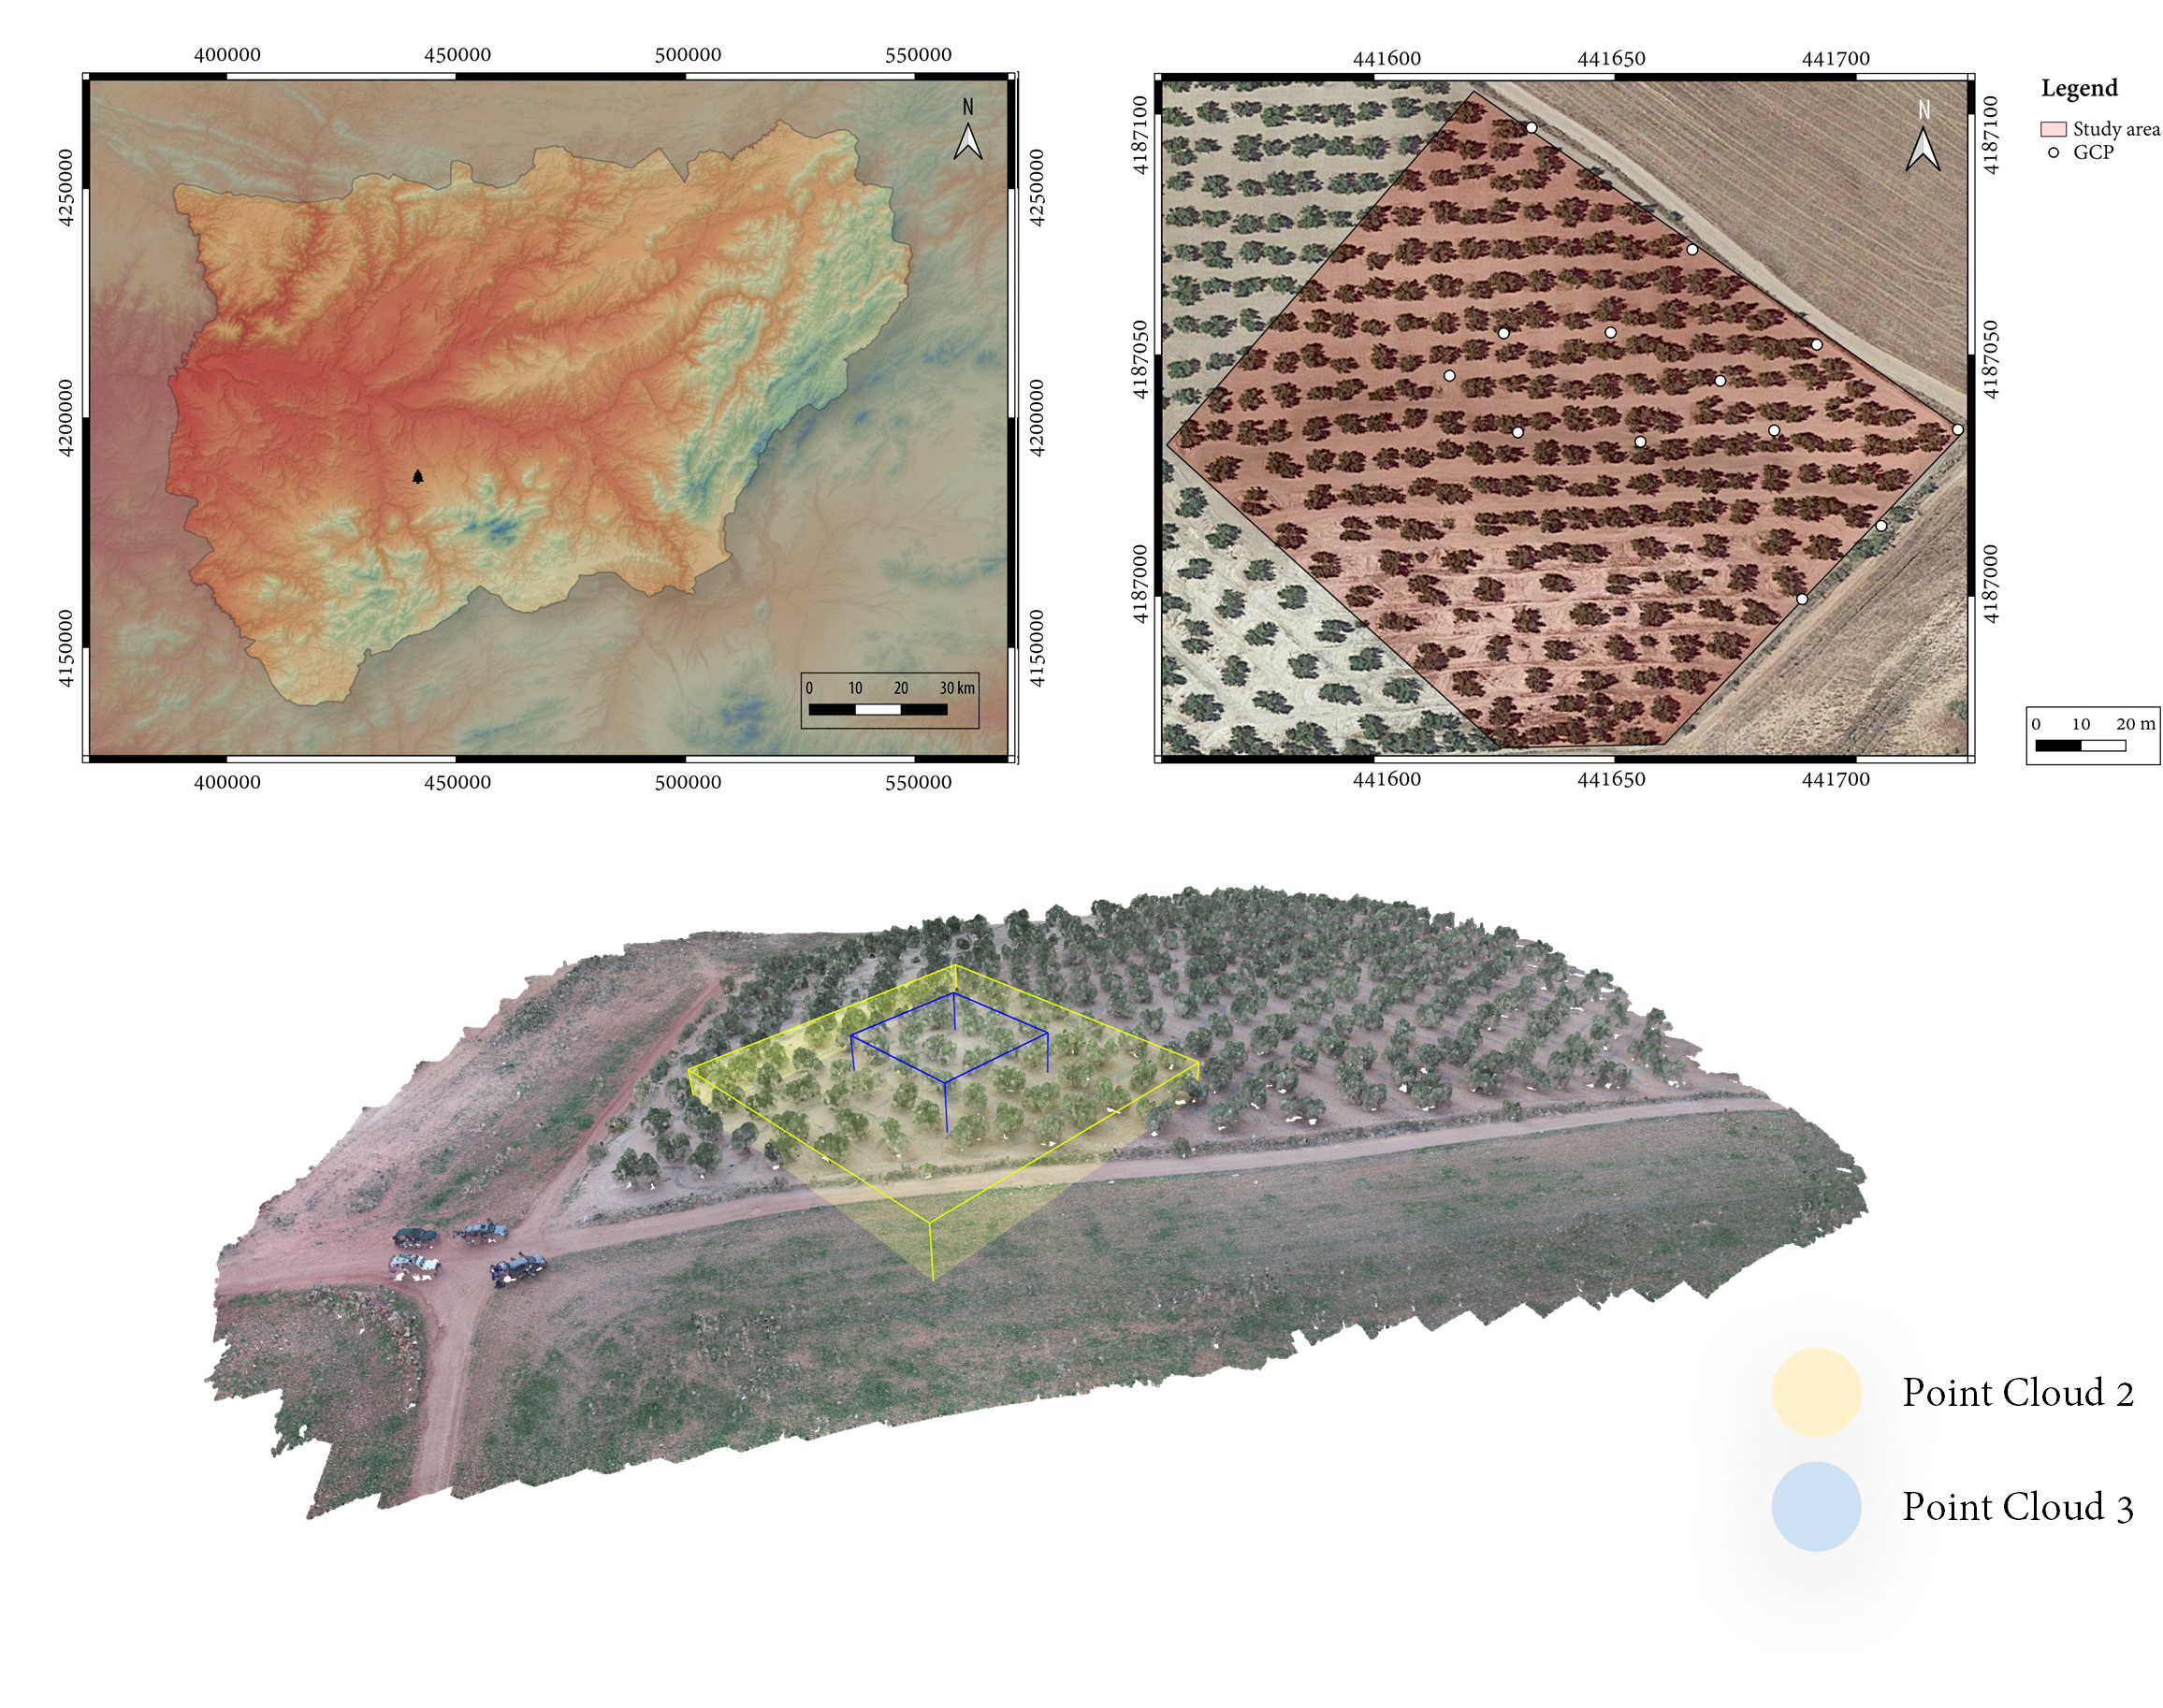
\includegraphics[width=\linewidth]{figs/thermal_projection/study_area_overview.png}
    \caption{An overview of the study area. On the left side, the location of the surveyed area in the region of Jaén, whereas the right side shows the study area as a portion of an olive grove. Coordinates are given in WGS84 (EPSG:4326). }
	\label{fig:thermal_study_area}
\end{figure*}

\subsection{Performance of thermal point cloud reconstruction}

An RGB point cloud of size 98,016,324 was used as input to assess the performance of three versions of this work: naive mapping, visibility-based mapping and occlusion-based mapping (focused on solving surface collisions in the GPU). Commercial software is, on the other hand, fed only with a thermographic image dataset. Two different search radii were evaluated: $r_1 \gets 20$ \si{\meter} and $r_2 \gets 30$ \si{\meter}, centred at $y = \frac{\textit{aabb}_{\textit{min}_{y}} + \textit{aabb}_{\textit{max}_{y}}}{2}$ for every image viewpoint, provided that $\textit{aabb}_{\textit{max}_{y}}$ and $\textit{aabb}_{\textit{min}_{y}}$ are the \textit{Y}-axis coordinates of both maximum and minimum points of the point cloud's bounding box. The visibility test is configured so that the size of a depth buffer is equal to the size of the original RGB images ($4000 \times 3000$ pixels). The occlusion test builds BVHs using Morton codes of 30 bits sorted with the Radix Sort algorithm and determining the best-matching neighbour on the overlapping with a radius of 50. The obtained results are summarized in Table \ref{table:thermal_point_cloud_approaches}. The point cloud was measured by calculating its convex hull using the Delaunay triangulation \cite{shewchuk_delaunay_2002} minus the area of internal gaps. Finally, penalty and aggregation functions were omitted in these tests, thus utilizing the arithmetic mean to aggregate thermal samples. 

\renewcommand{\arraystretch}{1.2}
    \begin{table*}
    \caption{Performance comparison of the proposed methods. The reported values are averaged over five different executions. $r_1$ and $r_2$ correspond to a search radius of 20 \si{\meter} and 30 \si{\meter} respectively. The best results for each measure are highlighted in bold. Mapped images shows the number of thermal images that were successfully mapped into the point cloud. For our method, it shows the number of registered RGB-thermal pairs. For commercial software, images are excluded whether their parameters cannot be estimated or no features are detected. }
    \label{table:thermal_point_cloud_approaches}
    \begin{tabular}{@{}lrrrr@{} }
    \toprule
    & \multicolumn{4}{c}{\textbf{Mapping approach}} \\
    \cmidrule{2-5}
    Attributes & Naive ($r_1$) & Depth buffer ($r_1$) & Occlusion ($r_1$) & Pix4Dmapper\\
    \midrule
    \#Points & 82.743.078 points & 79.511.469 points & 74.181.776 points & 9.782.277 points\\
    Area & 1,9973 ha & 1,9973 ha & 1,9973 ha & 1,9942 ha\\
    Point density & \textbf{4.143 points/\si{\metre\squared}} & 3.981 points/\si{\metre\squared} & 3.714 points/\si{\metre\squared} & 461 points/\si{\metre\squared}\\
    Response time & \textbf{3m 36,54s} & 7m 12,18s & 4m 27,83s & 13m 4,4s\\
    Response time/point & \textbf{2,617 \si{\micro\second}} & 5,435 \si{\micro\second} & 3,61 \si{\micro\second} & 80.185 \si{\micro\second}\\
    \#Mapped images & 368 of 410 & 368 of 410 & 368 of 410 & \textbf{371 of 410}\\[1mm]
    \cmidrule{2-5}
     & Naive ($r_2$) & Depth buffer ($r_2$) & Occlusion ($r_2$) & Agisoft Metashape\\
    \midrule
    \#Points & \textbf{82.767.436 points} & 79.511.469 points & 74.213.254 points & 18.045.885 points \\
    Area & \textbf{1,9991 ha} & \textbf{1,9991 ha} & \textbf{1,9991 ha} & 1,7202 ha \\
    Point density & 4.140 points/\si{\metre\squared} & 3.981 points/\si{\metre\squared} & 3.712 points/\si{\metre\squared} & 1.102 points/\si{\metre\squared} \\
    Response time & 7m 31,01s & 12m 4,38s & 9m 24,92s & 3m 48,31s \\
    Response time/point & 5,449 \si{\micro\second} & 5,435 \si{\micro\second} & 7,61 \si{\micro\second} & 12,113 \si{\micro\second} \\
    \#Mapped images & 368 of 410 & 368 of 410 & 368 of 410 & 326 of 410\\
    \bottomrule
    \end{tabular}
\end{table*}
\renewcommand{\arraystretch}{1}

\textbf{Number of points}. Thermal point clouds generated using the proposed method had the highest number of points. Despite this metric not reflecting the quality of the result, the geometry was indeed more accurate as it was obtained from an RGB reconstruction optimized with the marking of GCPs. In comparison, point clouds reconstructed solely from thermal data lacked point density and spatial covering due to the scarce tie-points that were obtained with SfM, as reported both in Table \ref{table:thermal_point_cloud_approaches} and Figure \ref{fig:thermal_point_cloud_comparison}. The naive approach discards $\sim16$M points which were not visible in any thermal image, whereas the number of points using $r_2$ increased by 358,64\% and 746,09\% with respect to Agisoft Metashape and Pix4Dmapper results. Occlusion-based approaches built point clouds of lower size with a radius equivalent to the GSD, although they greatly improved the result of commercial software. On the other hand, incrementing the radius size ($r_2 \rightarrow r_1$) barely improved the number of points whereas the latency significantly increased; hence, $r_1$ is preferred to $r_2$.

\textbf{Area and point density}. The proposed algorithm generated larger results regarding the covered area. Agisoft Metashape failed at the boundaries, while Pix4Dmapper results were very similar to ours despite having gaps (see Figure \ref{fig:thermal_point_cloud_comparison}). Additionally, the larger number of points also provided an advantageous point density. Consequently, the highest point density (from the naive mapping) increased the density by 275,95\% and 798,69\% with respect to Agisoft Metashape and Pix4Dmapper. As a reference, Javadnejad et al. \cite{javadnejad_photogrammetric_2020} obtained thermal point clouds with a density of 270 points/\si{\meter\squared} (0.36\si{\hectare} and 95 images), 336 points/\si{\meter\squared} (2.38\si{\hectare} and 101 images) and 5,429 points/\si{\meter\squared} (0,35\si{\hectare} and 165 images), while Webster et al. \cite{webster_three-dimensional_2018} operated with thermal datasets of 776 points/\si{\meter\squared}. The point density could be indeed improved by increasing the dataset dimensionality.

\textbf{Absolute and normalized response time}. The naive approach had the lowest latency, whereas occlusion-based methods were also quite competitive, despite Pix4Dmapper and Agisoft Metashape processing operating in CUDA-compatible GPUs. As previously described, the naive and depth buffer mapping algorithms were developed as sequential algorithms, while occlusion mapping utilized GPU for solving the collisions. The naive approach shows a small improvement in the overall response time in comparison with Agisoft Metashape, although the normalized response time outperforms commercial software (78,39\% and 96,73\% less processing time per point with respect to Agisoft Metashape and Pix4Dmapper, respectively). Results of occlusion mapping for $r_1$ were also remarkable as this algorithm required building a BVH for every image, each one integrating up to 6M points ($r_2$ peaks on 14,5 million points). 

\subsection{Aggregation of thermal data}

The proposed methodology was evaluated in order to prove its accuracy when assigning thermal values to 3D points. This chapter is relevant for aggregating thermal samples that carry different data due to being acquired from distinct viewing angles. The improvement of applying penalty functions was assessed by measuring the dissimilarity of aggregated values with respect to the imagery values. For that purpose, this variation was computed through the Root Mean-Square Deviation (RMSE), Mean Absolute Error (MAE) and standard deviation. However, penalty functions were applied as local optimizers where the result of a single aggregation was selected as the optimal one that minimizes a distance function (the penalty metric). This suggests that global measurements are not appropriate to account for aggregation-based results. Instead, the average RMSE and MAE (Equations \ref{eq:averaged_rmse_mae_avg_01} and \ref{eq:averaged_rmse_mae_avg_02}) are two criteria that are frequently used for unbalanced sets with a few items. Nonetheless, they enable quantifying the quality of the projected thermal data by measuring their distance to the image samples.
\begin{align*}
    \textit{RMSE} &= \sqrt{\frac{\sum_{i=1}^{p} \sum_{j=1}^{s_i} (S_j - A_i)^2}{\sum_{i=1}^{p} s_i}}     
    \numberthis \label{eq:averaged_rmse_mae_avg_01}\\
    \textit{MAE} &= \frac{\sum_{i=1}^{p} \sum_{j=1}^{s_i} \abs{S_j - A_i}}{\sum_{i=1}^{p} s_i} 
    \numberthis \label{eq:averaged_rmse_mae_avg_02}
\end{align*}
where $s_i$ is the number of samples ($S_j$) from where $A_i$ was calculated. Nevertheless, global RMSE and MAE were also annotated in Table \ref{table:thermal_error_dispersion}. RMSE and MAE equations were adapted to the point sets in this work as follows (Equations \ref{eq:rmse_mae_avg_01} and \ref{eq:rmse_mae_avg_02}):
\begin{align*}
    \textit{RMSE} &= \sqrt{\frac{\sum_{i=1}^{p} \sum_{j=1}^{s_i} (S_j - A_i)^2}{\sum_{i=1}^{p} s_i}}
    \numberthis \label{eq:rmse_mae_avg_01}\\
    \textit{MAE} &= \frac{\sum_{i=1}^{p} \sum_{j=1}^{s_i} \abs{S_j - A_i}}{\sum_{i=1}^{p} s_i}
    \numberthis \label{eq:rmse_mae_avg_02}
\end{align*}

Likewise, the average standard deviation of samples for each 3D point is shown in Equation \ref{eq:average_std}, provided that it does not consider the aggregated value regardless of penalty functions. 
\begin{align*}
    &\sigma_{\textit{mean}} = \frac{\sum_{i=1}^{p} \frac{\sum_{j=1}^{s_i} \abs{S_j - \{\overline{S_{i_0},...,S_{i_{s_i-1}}}\}}}{s_i}}{p} 
    \numberthis \label{eq:average_std}
\end{align*}

With the given definitions of penalty functions, $P_1$ and $P_2$ (see Table \ref{table:thermal_error_dispersion}), it can be observed that averaged RMSE and MAE are biased towards both functions. Nevertheless, penalty functions were included to minimize the sample dissimilarity, and despite this bias existing, it shows that penalty functions reduce the distance from the aggregated value to the set of image samples. Moreover, methods that checked occlusion and visibility were expected to obtain better results for averaged measures, as their number of samples is lower. However, global RMSE and MSE worsened the results of the penalty-based methods since the minimization was applied for $s_i$, instead of the overall number of samples, $\sum_{i=1}^{p} s_i$. The best value regarding the averaged RMSE was achieved by Occlusion-$P_2$, whereas Occlusion-$P_1$ lowers the distance measured by the averaged MAE. In any case, the penalty-based approaches improved the results of those approaches that solely used the arithmetic mean. The penalty function $P_1$ minimized the absolute error ($\textit{MAE}_{\textit{avg}}$), although penalty functions $P_2$ and $P_3$ penalized higher variations and thus minimized $\textit{RMSE}_{\textit{avg}}$.

The results of aggregating thermal data were assessed by computing the distance between histograms of 2D and 3D points. Although image samples were very different from each other, penalty functions were evaluated to check whether they produced variations in distance metrics. For that purpose, three conventional criteria were used to compare histograms, from the Pearson correlation coefficient (Equation \ref{eq:pearson_correlation}) to the Hellinger distance (Equation \ref{eq:hellinger_distance}) and intersection distance (Equation \ref{eq:intersection_distance}) \cite{cha_comprehensive_2007}. From now on, we will refer to them as $d_{\textit{pearson}}$, $d_{\textit{hellinger}}$ and $d_{\textit{intersection}}$ for the sake of simplicity. $d_{\textit{pearson}}$ coefficient ranges from -1 to 1, with 1 being a perfect correlation. Zero implies there exists no linear correlation and -1 indicates a perfect negative correlation. On the other hand, $d_{\textit{hellinger}}$ measures the similarity of two probability functions, where 1 implies that both distributions are orthogonal. The expression of Equation \ref{eq:hellinger_distance} is simplified if histograms $h_1$ and $h_2$ are defined as density functions in [0, 1] ($h_{\textit{norm}_{1_{i}}}$, $h_{\textit{norm}_{2_{i}}}$). Finally, the intersection, $d_{\textit{intersection}}$, is another widely used form of similarity for probability distributions. It returns 1 when $h_{\textit{norm}_{1_{i}}}$ and $h_{\textit{norm}_{2_{i}}}$ are completely overlapped. 
\begin{align*}
    d(h_1, h_2) &= \frac{\sum_{i=1}^{n} (h_{1_{i}} - \overline{h}_{1}) (h_{2_{i}} - \overline{h}_{2})}{\sqrt{\sum_{i=1}^{n} (h_{1_{i}} - \overline{h}_{1})^2 \sum_{i=1}^{n} (h_{2_{i}} - \overline{h}_{2})^2}}
    \numberthis \label{eq:pearson_correlation}\\
    d(h_1, h_2)
    &=\sqrt{1 - \frac{1}{\sqrt{\overline{h}_1 \overline{h}_2 \textit{n}^2}} \sum_{i=1}^{n} \sqrt{h_{1_{i}}h_{2_{i}}}}\\
    &=\sqrt{1 - \sum_{i=1}^{n} \sqrt{h_{norm_{1_{i}}}h_{norm_{2_{i}}}}}
    \numberthis \label{eq:hellinger_distance}\\
    d(h_1, h_2)
    &=\sum_{i=1}^{n} \min(h_{1_{i}}, h_{2_{i}})
    \numberthis \label{eq:intersection_distance}
\end{align*}
where $n$ is the number of bins of the histograms $h_1$ and $h_2$, both with the same dimensionality.

\begin{figure*}
    \centering
    \includegraphics[width=\linewidth]{figs/thermal_projection/histogram_composition.png}
	\caption{Intensity distribution for image samples used in the generation of the thermal point cloud, as well as the distributions obtained after applying two mapping methods (naive (no penalty) and naive (penalty-based, $P_3$)). The density functions concerning other approaches were omitted as they returned very similar results. Finally, the similarity between histograms was reported for each configuration, with minor changes in the distribution being highlighted. For the sake of simplicity, Hellinger distance was expressed as $1 - d$ to visualize the three metrics in the same chart. Hence, a value of 1 indicates that both histograms are equal ($h_{1_{i}} = h_{2_{i}}, \forall i \in [0, n)$), while 0 denotes complete dissimilarity ($h_{1_{i}} = 1 - h_{2_{i}}, \forall i \in [0, n)$).}
	\label{fig:thermal_histogram_results}
\end{figure*}

Figure \ref{fig:thermal_histogram_results} compares the source histogram for the naive approach and the histograms obtained from two mapping procedures (without penalty function and using $P_3$). The rest of the approaches obtained similar results and thus were omitted in this comparison. These slight variations were highlighted using the similarity metrics in Figure \ref{fig:thermal_histogram_results}. Remark that $d_{\textit{hellinger}}$ was transformed into $1 - d_{\textit{hellinger}}$ to visualize the three of them in the same interval. According to the reported results, occlusion-based methods obtained more similar results to the baseline histogram, especially for the occlusion test. Furthermore, the penalty function $P_1$, which computes the dispersion as $\abs{x_i - y}$, improved the baseline result for every approach.

\subsection{Analysis of thermal point cloud}

\begin{marginfigure}[1cm]
	\centering
	\includegraphics{figs/thermal_projection/temperature_class.png}
	\caption{Frequency function of thermal radiation for three-dimensional ground and vegetation points.}
	\label{fig:thermal_temperature_class}
\end{marginfigure}
The temperature of ground and vegetation points was retrieved and depicted in Figure \ref{fig:thermal_temperature_class} for a point cloud of $\sim90$M points. Accumulated values were presented as a density function based on the point cloud size. Although Figure \ref{fig:thermal_point_cloud_top_view} shows that vegetation presented an overall lower thermal radiation, both temperature datasets were far from being disjoint. Note that the vegetation class also includes low vegetation which was classified as anomalous hot regions. On the other hand, ground points also covered regions shadowed by trees. However, both distributions have a clearly distinct peak. Most thermal values ranged from 12 \textdegree C to 23 \textdegree C; anomalous hot regions were mainly identified in low vegetation and metallic surfaces, with cold regions being mainly observed at points belonging to some trees and ground.

\renewcommand{\arraystretch}{1.2}
\begin{table*}[ht]
    \caption{Dissimilarity of aggregated thermal data and 2D thermal samples, without accounting for occluded samples. Errors were computed using values that ranged from 0 to 1. }
    \label{table:thermal_error_dispersion}
    \begin{tabular}{@{}llrrrrr@{}}
    \toprule
    & & \multicolumn{5}{c}{\textbf{Metric}} \\
    \cmidrule{3-7}
    \textbf{Penalty function} & \textbf{Mapping algorithm} & Average $\sigma$ & Average RMSE & RMSE & Average MSE & MSE\\
    \midrule
    \multirow{3}{*}{No penalty} & Naive & 0.052 & 0.054 & \textbf{0.052} & 0.045 & 0.024\\
    & Visibility & 0.049 & 0.050 & 0.055 & 0.042 & 0.027\\
    & Occlusion & \textbf{0.039} & \textbf{0.042} & 0.054 & 0.042 & 0.054\\
    \midrule
    \multirow{3}{*}{$P_1 : \abs{d(x_i, y)}$} & Naive & 0.052 & 0.054 & 0.053 & 0.044 & \textbf{0.024} \\
    & Visibility & 0.049 & 0.051 & 0.055 & 0.041 & 0.027 \\
    & Occlusion & \textbf{0.039} & 0.042 & 0.055 & \textbf{0.035} & 0.034 \\
    \midrule
    \multirow{3}{*}{$P_2 : d(x_i, y)^2$} & Naive & 0.052 & 0.053 & \textbf{0.052} & 0.044 & \textbf{0.024} \\
    & Visibility & 0.049 & 0.050 & 0.054 & 0.042 & 0.027 \\
    & Occlusion & \textbf{0.039} & \textbf{0.041} & 0.053 & \textbf{0.036} & 0.035\\
    \midrule
    \multirow{3}{*}{$P_3 : \abs{d(x_i, y)}^3$} & Naive & 0.052 & 0.054 & \textbf{0.052} & 0.045 & \textbf{0.024} \\
    & Visibility & 0.049 & 0.050 & 0.054 & 0.043 & 0.027 \\
    & Occlusion & \textbf{0.039} & \textbf{0.041} & 0.053 & \textbf{0.037} & 0.035 \\
    \bottomrule
    \end{tabular}
\end{table*}
\renewcommand{\arraystretch}{1}

\subsection{Visualization of the point cloud}

A better insight into the reconstructed point clouds is provided by Figure \ref{fig:thermal_point_cloud_comparison}. It depicts three results (b, c and d): the first one is computed using the naive approach, while the other two are the outcome of Agisoft Metashape and Pix4Dmapper software. The result of Pix4Dmapper has some gaps as a result of images not being aligned due to the lack of key points. Furthermore, canopies were poorly estimated in comparison with the RGB reconstruction. On the other hand, the result of Agisoft Metashape shows a wide number of shortcomings. First, canopies were wrongly estimated and they were represented as planar surfaces. Moreover, a significant part of the study area had a wrong altitude besides other noticeable outliers. Sparsity concerns both point clouds, although it was considerably more significant for the Pix4Dmapper result, as reported in Table \ref{table:thermal_point_cloud_approaches}. Finally, the preservation of image details can be observed in Figure \ref{fig:thermal_zoomed_up}.

\begin{figure}[hbt]
	\centering
    \includegraphics[width=\linewidth]{figs/thermal_projection/thermal_close_view.png}
	\caption{Close-up view of a thermal point cloud with $\sim20$ million points. Details of thermal images are preserved and no blurring effects are observed.}
	\label{fig:thermal_zoomed_up}
\end{figure}

\section{Conclusions and future work}
\label{Conclusions and future work}

An efficient algorithm for building dense thermal point clouds was proposed in this chapter. RGB point clouds were used as input for providing results with a larger number of points (up to 798,69\% more points than commercial software). GPU-based algorithms were used to fasten some of the proposed algorithms, thus obtaining a decrease of 78,39\% in the processing time per 3D point in comparison with Agisoft Metashape. An innovative solution for the aggregation of multiple thermal samples was also proposed to minimize the dissimilarity of thermal and image intensity. Dispersion and histogram distance metrics showed that penalty functions clearly help in this task.

\begin{figure*}[htb]
    \centering
    \includegraphics[width=\linewidth]{figs/thermal_projection/thermal_visualization_comparison.png}
	\caption{a) Original RGB point cloud, retrieved with the original resolution, b) thermal point cloud computed using the naive approach, c) Agisoft Metashape result and 4) Pix4Dmapper result. }
	\label{fig:thermal_point_cloud_comparison}
\end{figure*}

This methodology is appropriate as an alternative to the traditional SfM-MVS algorithm. The latter is based on extracting features from images, which are harder to obtain from thermography. Instead, the RGB point cloud generated by SfM can be used as the baseline for projecting imagery. Also, the density of the point clouds estimated by our algorithm was higher and thus it could be more suitable for applications that require dense results, e.g., rendering software. Similarly, it operates as an efficient solution that helps in reducing latency.

\marginnote[1cm]{The ECC image matching can be barely improved from here. However, the acquisition of thermal images was performed so that visual information is obtained by fusing infrared and RGB data. Although it may help on some datasets, the included edges were very fuzzy for vegetation. Hence, disabling this overlapped data may help in the image-matching task. } 
This chapter leaves some open questions that will be addressed in later chapters or remains as future work. Firstly, in-situ radiometric calibration may help on shedding light on the accuracy of the temperature estimation. From here, a reliable multi-temporal system could be proposed over reconstructed thermal point clouds for the analysis of individual trees. As previously stated, the target area was partly affected by the \textit{Xylella fastidiosa} pathogen and thus could be monitored using thermography. The registration of RGB and thermal images could also be improved to increase the point density of resulting point clouds. Finally, more competitive solutions concerning efficiency could be developed by implementing the entire workflow in GPU, which is the topic of the following chapter. This study could be further extended to compare several parallel-computing frameworks and take advantage of rendering tools, such as OpenGL's built-in \textit{z}-buffer.